% %%%%%%%%%%%%%%%%%%%%%%%%%%%%%%%%%%%%%%%%%%%%%%%%%%%%%%%
% Please note that whilst this template provides a 
% preview of the typeset manuscript for submission, it 
% will not necessarily be the final publication layout.
%
%% Document class options: (**...** are defaults)
%  - bibtex: Uses bibtex+natbib, chicago.bst 
%  - biblatex: Uses biblatex-chicago
%      You MUST select one of the above two options, depending
%      on whether you prefer bibtex or biblatex. This template
%      contains code that uses bibtex.
%  - twocolumn: Switch to two column for main text
%  - singlespace/onehalfspace/**doublespace**: 
%         changes line spacing for main text
%  - **blind**/nonblind: Anonymises authors 
%         and affiliations, or not
%  - autowc: Automatically inserts a word count
%         after the abstract, using texcount. 
%         The abstract is ignored. 
%         NOTE THAT THIS WILL ONLY WORK IF YOU HAVE  
%         INSTALLED TEXCOUNT, AND HAVE ENABLED --shell-escape
%         OR --enable-write18. (These will work on Overleaf.)
%         If you get an error about "texcount not found", delete
%         the autowc option, and manually specify the wordcount 
%         with \totalwordcount{xxx}.
%%% autowc may cause longer compilation time. You can 
%%% disable it first while actively editing, and only
%%% enable it when you're ready to take stock and check
%%% on your work.
\documentclass[bibtex,autowc]{apsr_submission}
% \totalwordcount{500}

%% Example alternative options with everything the opposite of the above: (DO NOT USE AUTOWC WITH BIBLATEX; the word count will be greatly over-reported)
% \documentclass[biblatex,nonblind,singlespace,twocolumn]{apsr_submission}

\title{American Political Science Review \emph{(APSR)} Submission Template}

% The custom \author command takes THREE arguments:
% #1 = Author name
% #2 = Affiliation name
% #3 = Brief author profile, or anything that you'd usually put in a \thanks. Leave blank {} if there's nothing to be said.
\author{Author One}
       {Affiliation A}
       {Author One is PhD Candidate, ABC Department, Affiliation A, 12345 NY. (a.1@example.edu)}
       
\author{Author Two}
       {Affiliation C}
       {Author Two is Assistant Professor, Faculty of Z, Affiliation B, 42813. Corresponding Author (a.2@acme.edu) Additional notes about Author Two.}
       
\author{Author Three}
       {Affiliation B}
       {Author Three is ...}

%% Any other acknowledgements or author notes
\thanks{The authors thank...}

%% These are used for the headers
\runningtitle{APSR Submission Template}
\runningauthor{Author One, Author Two, and Author Three} % 4 + Authors, Author One et al. 

%% Useful packages
\usepackage{amsmath}
\usepackage{graphicx}
\usepackage{rotating}

%% If you are using a custom figure or table environment from a package and it's not getting framed, add \makeframedenv{MyFigure} in the preamble, where the custom figure environment is \begin{MyFigure}...\end{MyFigure}.
%% Currently table, table*, figure, figure*, longtable, supertabular, sidewaystable and sidewaysfigure will be automatically framed.

%% Handy for setting wide tables/figures in landscape
\usepackage{pdflscape}

%% Recent LaTeX distributions should be able to automatically convert .eps to .pdf; but if this isn't happening, try loading the epstopdf package manually
% \usepackage{epstopdf}

%% Just to add some dummy text
\usepackage{lipsum}

%%% Use \addbibresource{...} if using BibLaTeX
% \addbibresource{sample.bib}

\begin{document}
%%% DO NOT REMOVE THESE LINES. For automatic word count.
%TC:ignore
\begin{frontmatter}
\begin{abstract}
Your abstract. It should be at least three lines long to accommodate the dropped-cap. \lipsum[1]
\end{abstract}
\end{frontmatter}
%%% DO NOT REMOVE THIS LINE. For automatic word count.
%TC:endignore

\section{Introduction}

\dropcap{Thanks} for using Overleaf to write your article. Your introduction goes here! Do make sure the first paragraph here is at least three lines long, to accommodate the dropped-cap. Some examples of commonly used commands and features are listed below, to help you get started.

Here's a second paragraph of extra text, to test paragraph indents.

\section{Some \LaTeX{} Examples}
\label{sec:examples}

Use section and subsection commands to organize your document. \LaTeX{} handles all the formatting and numbering automatically. Use \verb|\ref| and \verb|\label| commands for cross-references.

\subsection{Figures and Tables}

Use the table and tabular commands for basic tables --- see Table \ref{tab:widgets}, for example. \href{http://tablesgenerator.com}{TablesGenerator.com} is a handy tool for designing tables and generating the  LaTeX code, which you can copy and paste into your article here.

You can upload a figure (JPG, PNG or PDF) using the PROJECT menu (Files\ldots > Add files). To include it in your document, use the \verb|graphicx| package and the \verb|\includegraphics| command as in the code for Figure \ref{fig:view}. 

\begin{table}[hbt!]
\caption{An example table}
\label{tab:widgets}
\centering
\begin{tabular}{lr}
Item & Quantity \\\midrule
Widgets & 42 \\
Gadgets & 13
\end{tabular}
\floatnote{This is a note for this table.}
\end{table}

\begin{figure}[hbt!]

\includegraphics[width=\linewidth]{example-image}
\caption{A figure example.}
\label{fig:view}

\floatnote{This is a note for this figure.}
\end{figure}


Notes can be added to the bottom of figures and tables using the \verb|\floatnote| command.


\begin{table*}
\caption{Automobile Land Speed Records (GR 5-10).}
\label{tab:wide}

\begin{tabular}{l l l l r}
Speed (mph) & Driver          & Car                        & Engine    & Date     \\
\midrule
407.447     & Craig Breedlove & Spirit of America          & GE J47    & 8/5/63   \\
413.199     & Tom Green       & Wingfoot Express           & WE J46    & 10/2/64  \\
434.22      & Art Arfons      & Green Monster              & GE J79    & 10/5/64  \\
468.719     & Craig Breedlove & Spirit of America          & GE J79    & 10/13/64 \\
526.277     & Craig Breedlove & Spirit of America          & GE J79    & 10/15/65 \\
536.712     & Art Arfons      & Green Monster              & GE J79    & 10/27/65 \\
555.127     & Craig Breedlove & Spirit of America, Sonic 1 & GE J79    & 11/2/65  \\
576.553     & Art Arfons      & Green Monster              & GE J79    & 11/7/65  \\
600.601     & Craig Breedlove & Spirit of America, Sonic 1 & GE J79    & 11/15/65 \\
622.407     & Gary Gabelich   & Blue Flame                 & Rocket    & 10/23/70 \\
633.468     & Richard Noble   & Thrust 2                   & RR RG 146 & 10/4/83  \\
763.035     & Andy Green      & Thrust SSC                 & RR Spey   & 10/15/97\\
\end{tabular}

\floatnote{\url{https://www.sedl.org/afterschool/toolkits/science/pdf/ast_sci_data_tables_sample.pdf}}

\end{table*}

For wide, double-column figures and tables, use the \verb|figure*| (Figure \ref{fig:wide}) or \verb|table*| (Table \ref{tab:wide}) starred environments. Landscaped figures and tables can be obtained using the \texttt{sidewaysfigure} and \texttt{sidewaysfigure} commands from the \texttt{rotating} package. Alternatively, you can use the \texttt{landscape} environment from the \texttt{pdflscape} package.

Multi-page tables can be created using the \texttt{longtable} and \texttt{supertabular} packages, though note that \texttt{longtable}s cannot be used in two-column documents.\footnote{This is an example footnote. \lipsum[1]}


Currently \texttt{table}, \texttt{table*}, \texttt{figure}, \texttt{figure*}, \texttt{longtable}, \texttt{supertabular}, \texttt{sidewaystable} and \texttt{sidewaysfigure} will be automatically framed.

If you are using a custom figure or table environment from a package (e.g.~a \texttt{MyFigure} environment) and it's not getting framed, add \verb|\makeframedenv{MyFigure}| in the preamble. 

\subsection{Lists and Quotations}

You can make lists with automatic numbering \dots

\begin{enumerate}
\item Like this,
\item and like this.
\end{enumerate}

\dots or bullet points \dots

\begin{itemize} 
\item Like this,
\item and like this.
\end{itemize}

\dots or with words and descriptions \dots

\begin{description}
\item[Word] Definition
\item[Concept] Explanation
\item[Idea] Text
\end{description}

An example quotation:

\begin{quoting}
This is a sample quotation text. This is a sample quotation text. This is a sample quotation text.
\end{quoting}

(This is some filler text.) \lipsum[2]

\subsection{Citations}

\LaTeX{} formats citations and references automatically using the bibliography records in your .bib file, which you can edit via the project menu. Use the \verb|\citep| command for a citation in parentheses \citep{greenwade93}, or  \verb|\citet| for a text citation: \citet{greenwade93}. Multiple citations can be given as \citep{greenwade93,knuth1984texbook}.

If your manuscript is accepted, the APSR production team will re-format the references for publication. \emph{It is not necessary to format the reference list yourself to mirror the final published form.}

\subsubsection{Using bibtex} Pass the \texttt{bibtex} option to the \verb|\documentclass| declaration, then specify your \texttt{.bib} file with \verb|\bibliography{sample}| (the extension is unnecessary) near the end of your manuscript, where you want the references list to appear.

\subsubsection{Using biblatex} Pass the \texttt{biblatex} option to the \verb|\documentclass| declaration, then specify your \texttt{.bib} file name in the \emph{preamble}: \verb|\addbibresource{sample.bib}| (the extension is necessary). Write \verb|\printbibliography| near the end of your manuscript where you want the references to appear.

Note that you may want to remove the \texttt{autowc} (automatic word count) document class option, if you are using \texttt{biblatex}. There have been reports of texcount over-reporting word counts when authors use \texttt{biblatex}, due to the database nature of \texttt{.bbl} files produced by \texttt{biblatex}. For more information, see \url{https://tex.stackexchange.com/a/110902/226}.

\subsection{Mathematics}

\LaTeX{} is great at typesetting mathematics:

Let $X_1, X_2, \ldots, X_n$ be a sequence of independent and identically distributed random variables with $\text{E}[X_i] = \mu$ and $\text{Var}[X_i] = \sigma^2 < \infty$, and let
\begin{equation}
\label{eq:CLT}
S_n = \frac{X_1 + X_2 + \cdots + X_n}{n}
      = \frac{1}{n}\sum_{i}^{n} X_i
\end{equation}
denote their mean. Then as $n$ approaches infinity, the random variables $\sqrt{n}(S_n - \mu)$ converge in distribution to a normal $\mathcal{N}(0, \sigma^2)$.

\begin{figure*}
\centering
\caption{A wide figure}\label{fig:wide}
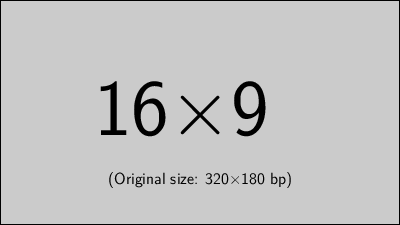
\includegraphics[width=\linewidth]{example-image-16x9}
\end{figure*}

\section{Level 1 heading}

\lipsum[2]

\subsection{Level 2 Heading}

\lipsum[3]

\subsubsection{Level 3 Heading}

\lipsum[4]
\begin{table*}[htp!] \centering \footnotesize
  \caption{Panel Linear Model of the Full Sample of Data to Show Long Tables} 
  \label{tab:plmdata} 
\begin{tabular}{@{\extracolsep{5pt}}lcccc} 

 & \multicolumn{4}{c}{\textsl{Dependent variable: $log(Dependent Variable_{t-1} + 1)$}} \\ 
\cline{2-5} 
\\[-1.8ex] & (1) & (2) & (3) & (4) \\ 
\hline \\[-1.8ex] 
  Variable q  & $-$0.512 & $-$0.674 & $-$0.421 & $-$0.374 \\ 
  & (0.510) & (0.525) & (0.517) & (0.537) \\ 
  Variable 2 & 1.108$^{***}$ & 0.798$^{***}$ & 0.784$^{***}$ & 0.703$^{**}$ \\ 
  & (0.288) & (0.283) & (0.275) & (0.288) \\ 
  Variable 3  & 0.200 & 0.202 & 0.304$^{**}$ & 0.285$^{**}$ \\ 
  & (0.138) & (0.139) & (0.139) & (0.138) \\ 
  Variable 4 &  & $-$0.766$^{***}$ & $-$1.036$^{***}$ & $-$0.982$^{***}$ \\ 
  &  & (0.254) & (0.255) & (0.251) \\ 
  Variable 5 &  & 0.120 & 0.232$^{*}$ & 0.260$^{*}$ \\ 
  &  & (0.127) & (0.134) & (0.138) \\ 
  Variable 6 &  & 0.341$^{***}$ & 0.395$^{***}$ & 0.357$^{***}$ \\ 
  &  & (0.071) & (0.072) & (0.072) \\  
  Variable 7 &  &  & 0.232$^{***}$ & 0.189$^{***}$ \\ 
  &  &  & (0.034) & (0.036) \\ 
  Variable 8 &  &  & 0.253$^{***}$ & 0.206$^{***}$ \\ 
  &  &  & (0.037) & (0.042) \\ 
  Variable 9 &  &  & 0.060$^{***}$ & 0.051$^{***}$ \\ 
  &  &  & (0.008) & (0.009) \\ 
  Variable 10 &  &  & $-$0.018$^{***}$ & $-$0.012$^{*}$ \\ 
  &  &  & (0.007) & (0.007) \\ 
  Variable 11 &  &  &  & 0.329$^{***}$ \\ 
  &  &  &  & (0.125) \\ 
  Variable 12 &  &  &  & $-$0.320$^{***}$ \\ 
  &  &  &  & (0.062) \\ 
  Variable 13 &  &  &  & $-$0.124$^{***}$ \\ 
  &  &  &  & (0.031) \\ 
  Variable 14 &  &  &  & $-$0.060 \\ 
  &  &  &  & (0.057) \\ 
  Variable 15 &  &  &  & $-$0.340$^{***}$ \\ 
  &  &  &  & (0.055) \\ 
  Variable 16 &  &  &  & $-$0.123$^{***}$ \\ 
  &  &  &  & (0.033) \\ 
  Variable 17 & 0.0002 & 0.001 & $-$0.001 & $-$0.0003 \\ 
  & (0.001) & (0.001) & (0.001) & (0.001) \\
  Variable 18 & 0.006$^{***}$ & 0.005$^{***}$ & 0.012$^{***}$ & 0.011$^{***}$ \\ 
  & (0.001) & (0.001) & (0.001) & (0.001) \\ 
  Variable 19 & $-$0.129$^{***}$ & $-$0.123$^{***}$ & $-$0.039 & $-$0.036 \\ 
  & (0.032) & (0.032) & (0.034) & (0.036) \\ 
  Variable 20 & 0.629$^{***}$ & 0.624$^{***}$ & 0.598$^{***}$ & 0.618$^{***}$ \\ 
  & (0.010) & (0.010) & (0.010) & (0.011) \\ 
  Constant & 0.275$^{***}$ & 0.946$^{***}$ & $-$2.334$^{***}$ & $-$1.017$^{**}$ \\ 
  & (0.056) & (0.298) & (0.439) & (0.475) \\ 

\hline \\[-1.8ex] 
Obs. & 32,658 & 32,658 & 32,658 & 28,200 \\ 
Adj. R$^{2}$ & 0.371 & 0.374 & 0.389 & 0.429 \\ 
F Stat. & 2,756.800$^{***}$  & 1,949.369$^{***}$  & 1,485.940$^{***}$  & 1,058.683$^{***}$  \\ 
\hline \\[-1.8ex] 
\textsl{Note:}  & \multicolumn{4}{l}{$^{*}$p$<$0.1; $^{**}$p$<$0.05; $^{***}$p$<$0.01} \\ 
\end{tabular} 
\end{table*}  

%% Use \bibliography{...} if using BibTeX
\bibliography{sample}

%TC:subst \printbibliography \bibliography
%TC:macro \field [0,1]
%TC:macro \name [0,0,0,1]
%TC:macro \list [0,0,1]
%% Use \printbibliography if using BibLaTeX
% \printbibliography

\end{document}